
We have used find\_package() extensively in previous chapters. We saw how convenient it is and how it simplifies the whole process. To make our project accessible through this command, we need to complete a few steps so that CMake can treat our project as a coherent package:

\begin{itemize}
\item 
Make our targets relocatable.

\item 
Install the target export file to a standard location.

\item 
Create a config-files and version file for the package.
\end{itemize}

Let's start from the beginning: why do targets need to be relocatable and how can we do this?

\subsubsubsection{11.4.1\hspace{0.2cm}Understanding the issues with relocatable targets}

Installation solves many problems but unfortunately, it also introduces some complexity: not only is CMAKE\_INSTALL\_PREFIX platform-specific but it can also be set by the user at the installation stage with the -{}-prefix option. However, target export files are generated before the installation, during the build stage, at which point we don't know where the installed artifacts will go. Take a look at the following code:

\begin{lstlisting}[style=styleCMake]
# chapter-11/01-export/src/CMakeLists.txt

add_library(calc STATIC calc.cpp)
target_include_directories(calc INTERFACE include)
\end{lstlisting}

In this example, we specifically add the include directory to the include directories of calc.
Since this is a relative path, CMake's exported target generation will implicitly prepend this path with the contents of the CMAKE\_CURRENT\_SOURCE\_DIR variable, which points to the directory where this listfile is located.

However, that's not going to cut it. The installed project shouldn't need files from the source or build tree anymore. Everything (including library headers) is copied to a shared location, such as /usr/lib/calc/ on Linux. We cannot use the target that's been defined in this snippet in another project since the target's include directory path still points to its source tree.

CMake solves this with two generator expressions that will filter out the expression, depending on the context:

\begin{itemize}
\item 
\$<BUILD\_INTERFACE>: This includes the content for regular builds but excludes it for installation.

\item 
\$<INSTALL\_INTERFACE>: This includes the content for installation but excludes it for regular builds.
\end{itemize}

The following code shows how you can use them in practice:

\begin{lstlisting}[style=styleCMake]
# chapter-11/06-install-export/src/CMakeLists.txt

add_library(calc STATIC calc.cpp)
target_include_directories(calc INTERFACE
	"$<BUILD_INTERFACE:${CMAKE_CURRENT_SOURCE_DIR}/include>"
	"$<INSTALL_INTERFACE:${CMAKE_INSTALL_INCLUDEDIR}>"
)
set_target_properties(calc PROPERTIES
	PUBLIC_HEADER src/include/calc/calc.h
)
\end{lstlisting}

For regular builds, the value of the calc target property, INTERFACE\_INCLUDE\_DIRECTORIES, will be expanded, like so:

\begin{tcblisting}{commandshell={}}
"/root/examples/chapter-11/05-package/src/include" ""
\end{tcblisting}

Empty double quotes mean that the value provided in INSTALL\_INTERFACE was excluded and evaluated as an empty string. On the other hand, when we install, the value will get expanded like so:

\begin{tcblisting}{commandshell={}}
"" "/usr/lib/calc/include"
\end{tcblisting}

This time, the value that was provided in the BUILD\_INTERFACE generator expression was evaluated as an empty string, and we're left with the value from the other generator expression.

One more word about CMAKE\_INSTALL\_PREFIX: this variable shouldn't be used as a component in paths specified in targets. It would be evaluated during the build stage, making the path absolute and not necessarily the same as the one that was provided in the installation stage (as users may use the -{}-prefix option). Instead, use the \$<INSTALL\_PREFIX> generator expression:

\begin{lstlisting}[style=styleCMake]
target_include_directories(my_target PUBLIC
	$<INSTALL_INTERFACE:$<INSTALL_PREFIX>/include/MyTarget>
)
\end{lstlisting}

Or, even better, you can use relative paths (they will get prepended with the correct installation prefix):

\begin{lstlisting}[style=styleCMake]
target_include_directories(my_target PUBLIC
	$<INSTALL_INTERFACE:include/MyTarget>
)
\end{lstlisting}

Please take a look at the official documentation for more examples and information (a link to this can be found in the Further reading section).

Now that our targets are "installation-compatible," we can safely generate and install their target export files.

\subsubsubsection{11.4.2\hspace{0.2cm}Installing target export files}

We discussed target export files a little bit in the Exporting without installation section.
Target export files that are intended for installation are quite similar, as is the signature of the command for creating them:

\begin{lstlisting}[style=styleCMake]
install(EXPORT <export-name> DESTINATION <dir>
		[NAMESPACE <namespace>] [[FILE <name>.cmake]|
		[PERMISSIONS permissions...]
		[CONFIGURATIONS [Debug|Release|...]]
		[EXPORT_LINK_INTERFACE_LIBRARIES]
		[COMPONENT <component>]
		[EXCLUDE_FROM_ALL])
\end{lstlisting}

It's a combination of "plain" export(EXPORT) and other install() commands (its options work the same way). Just remember that it will create and install a target export file for a named export that must be defined with the install(TARGETS) command. The major difference to be aware of here is that the generated export file will contain the target paths that were evaluated in the INSTALL\_INTERFACE generator expression and not BUILD\_INTERFACE like export(EXPORT) did.

In this example, we'll generate and install the target export file for the target from chapter-11/06-install-export/src/CMakeLists.txt. To do so, we must call install(EXPORT) in our top listfile:

\begin{lstlisting}[style=styleCMake]
# chapter-11/06-install-export/CMakeLists.txt

cmake_minimum_required(VERSION 3.20.0)
project(InstallExport CXX)
include(GNUInstallDirs) # so it's available in ./src/
add_subdirectory(src bin)

install(TARGETS calc EXPORT CalcTargets ARCHIVE
	PUBLIC_HEADER DESTINATION
		${CMAKE_INSTALL_INCLUDEDIR}/calc
)
install(EXPORT CalcTargets
	DESTINATION ${CMAKE_INSTALL_LIBDIR}/calc/cmake
	NAMESPACE Calc::
)
\end{lstlisting}

Again, note how we're referencing the CalcTargets export name in install(EXPORT).

Running cmake -{}-install in the build tree will result in the export file being generated in the specified destination:

\begin{tcblisting}{commandshell={}}
...
-- Installing: /usr/local/lib/calc/cmake/CalcTargets.cmake
-- Installing: /usr/local/lib/calc/cmake/CalcTargets-noconfig.cmake
\end{tcblisting}

If, for some reason, the override default name for the target export file (<export name>.cmake) doesn't work for you, you can add the FILE new-name.cmake argument to change it (the filename must end with .cmake).

Don't get confused by this – the target export file isn't a config file, so you can't use find\_package() to consume installed targets just yet. However, it's possible to include() export files directly if needed. So, how do we define the package that can be consumed by other projects? Let's find out!

\subsubsubsection{11.4.3\hspace{0.2cm}Writing basic config-files}

A complete package definition consists of the target export files, the package's config file, and the package's version file, but technically, all that's needed for find\_package() to work is a config-file. It's considered a package definition and it's responsible for providing any package functions and macros, checking requirements, finding dependencies, and including target export files.

As we mentioned earlier, users can install your package anywhere on their system by using the following command:

\begin{tcblisting}{commandshell={}}
cmake --install <build tree> --prefix=<installation path>
\end{tcblisting}

This prefix determines where the installed files will be copied. To support this, you must at least ensure the following:

\begin{itemize}
\item 
The paths on the target properties can be relocated (as described in the Understanding the issues with relocatable targets section).

\item 
The paths that are used in your config-file are relative to it.
\end{itemize}

To use such packages that have been installed in non-default locations, the consuming projects need to provide <installation path> through the CMAKE\_PREFIX\_PATH variable during the configuration stage. We can do this with the following command:

\begin{tcblisting}{commandshell={}}
cmake -B <build tree> -DCMAKE_PREFIX_PATH=<installation path>
\end{tcblisting}

The find\_package() command will scan the list of paths that are outlined in the documentation (link in the Further reading section) in a platform-specific way. One of the patterns that's checked on Windows and Unix-like systems is as follows:

\begin{tcblisting}{commandshell={}}
<prefix>/<name>*/(lib/<arch>|lib*|share)/<name>*/(cmake|CMake)
\end{tcblisting}

This tells us that installing the config-file in a path such as lib/calc/cmake should work just fine. Also, it's important to highlight that config-files must be named <PackageName>-config.cmake or <PackageName>Config.cmake to be found.

Let's add the installation of the config-file to the 06-install-export example:

\begin{lstlisting}[style=styleCMake]
# chapter-11/07-config-file/CMakeLists.txt (fragment)

...
install(EXPORT CalcTargets
	DESTINATION ${CMAKE_INSTALL_LIBDIR}/calc/cmake
	NAMESPACE Calc::
)
install(FILES "CalcConfig.cmake"
	DESTINATION ${CMAKE_INSTALL_LIBDIR}/calc/cmake
)
\end{lstlisting}

This command will install CalcConfig.cmake from the same source directory (CMAKE\_INSTALL\_LIBDIR will be evaluated to the correct lib path for the platform).

The most basic config-file we can provide consists of a single line that includes the target export file:

\begin{lstlisting}[style=styleCMake]
# chapter-11/07-config-file/CalcConfig.cmake

include("${CMAKE_CURRENT_LIST_DIR}/CalcTargets.cmake")
\end{lstlisting}

The CMAKE\_CURRENT\_LIST\_DIR variable refers to the directory that the config-file lives in. Because CalcConfig.cmake and CalcTargets.cmake are installed in the same directory in our example (as set by install(EXPORT)), the target export file will be included correctly.

To make sure that our package is usable, we'll create a simple project consisting of just one listfile:

\begin{lstlisting}[style=styleCMake]
# chapter-11/08-find-package/CMakeLists.txt

cmake_minimum_required(VERSION 3.20.0)
project(FindCalcPackage CXX)

find_package(Calc REQUIRED)
include(CMakePrintHelpers)
message("CMAKE_PREFIX_PATH: ${CMAKE_PREFIX_PATH}")
message("CALC_FOUND: ${Calc_FOUND}")
cmake_print_properties(TARGETS "Calc::calc" PROPERTIES
	IMPORTED_CONFIGURATIONS
	INTERFACE_INCLUDE_DIRECTORIES
)
\end{lstlisting}

To test this in practice, we can build and install the 07-config-file example to one directory, and then build 08-find-package while referencing it with the DCMAKE\_PREFIX\_PATH argument, like so:

\begin{tcblisting}{commandshell={}}
# cmake -S <source-tree-of-07> -B <build-tree-of-07>
# cmake --build <build-tree-of-07>
# cmake --install <build-tree-of-07>
# cmake -S <source-tree-of-08> -B <build-tree-of-08>
  -DCMAKE_PREFIX_PATH=<build-tree-of-07>
\end{tcblisting}

This will produce the following output (all the <\_tree-of\_> placeholders will be replaced with real paths):

\begin{tcblisting}{commandshell={}}
CMAKE_PREFIX_PATH: <build-tree-of-07>
CALC_FOUND: 1
--
  Properties for TARGET Calc::calc:
    Calc::calc.IMPORTED_CONFIGURATIONS = "NOCONFIG"
    Calc::calc.INTERFACE_INCLUDE_DIRECTORIES = 
      "<buildtree-of-07>/include"
-- Configuring done
-- Generating done
-- Build files have been written to: <build-tree-of-08
\end{tcblisting}

The CalcTargets.cmake file was found and included correctly, and the path to the include directory was set to follow the chosen prefix. This solves packaging for a very basic case. Now, let's learn how to handle more advanced scenarios.

\subsubsubsection{11.4.4\hspace{0.2cm}Creating advanced config-files}

If you have more things to manage than a single target export file, it might be useful to include a few macros in your config-file. The CMakePackageConfigHelpers utility module gives us access to the configure\_package\_config\_file() command. To use it, we need to supply a template file that will be interpolated with CMake variables to generate a config-file with two embedded macro definitions:

\begin{itemize}
\item 
set\_and\_check(<variable> <path>): This works like set(), but it checks that <path> actually exists and fails with FATAL\_ERROR otherwise. It is recommended to use this in your config-files to detect incorrect paths early.

\item 
check\_required\_components(<PackageName>): This is added to the end of the config-file and will verify whether all the components in our package, which are required by the user in find\_package(<package> REQUIRED <component>), have been found. This is done by checking that the <package>\_<component>\_FOUND variables are true.
\end{itemize}

Paths for more convoluted directory trees can be prepared for the installation stage while you're generating the config-file. Take a look at the following signature:

\begin{lstlisting}[style=styleCMake]
configure_package_config_file(<template> <output>
	INSTALL_DESTINATION <path>
	[PATH_VARS <var1> <var2> ... <varN>]
	[NO_SET_AND_CHECK_MACRO]
	[NO_CHECK_REQUIRED_COMPONENTS_MACRO]
	[INSTALL_PREFIX <path>]
	)
\end{lstlisting}

The file that's been provided as <template> will be interpolated with variables and stored in the <output> path. Here, the path that's required after INSTALL\_DESTINATION will be used to transform the paths stored in the variables listed in PATH\_VARS so that they are relative to the install destination. We can also indicate that INSTALL\_DESTINATION is relative to INSTALL\_PREFIX by providing it as its base path.

NO\_SET\_AND\_CHECK\_MACRO and NO\_CHECK\_REQUIRED\_COMPONENTS\_MACRO tell CMake not to add these macro definitions to the generated config-file. Let's see this generation in practice. Again, we'll extend the 06-install-export example:

\begin{lstlisting}[style=styleCMake]
# chapter-11/09-advanced-config/CMakeLists.txt (fragment)

...
install(EXPORT CalcTargets
	DESTINATION ${CMAKE_INSTALL_LIBDIR}/calc/cmake
	NAMESPACE Calc::
)

include(CMakePackageConfigHelpers)
set(LIB_INSTALL_DIR ${CMAKE_INSTALL_LIBDIR}/calc)
configure_package_config_file(
	${CMAKE_CURRENT_SOURCE_DIR}/CalcConfig.cmake.in
	"${CMAKE_CURRENT_BINARY_DIR}/CalcConfig.cmake"
	INSTALL_DESTINATION ${CMAKE_INSTALL_LIBDIR}/calc/cmake
	PATH_VARS LIB_INSTALL_DIR
)
install(FILES "${CMAKE_CURRENT_BINARY_DIR}/CalcConfig.cmake"
	DESTINATION ${CMAKE_INSTALL_LIBDIR}/calc/cmake
)
\end{lstlisting}

Let's take a look at what we must do in the preceding code:

\begin{enumerate}
\item 
include() the utility module with helpers.

\item 
set() a variable that will be used to make a relocatable path.

\item 
Generate the CalcConfig.cmake config-file for the build tree using the CalcConfig.cmake.in template located in the source tree. Finally, provide LIB\_INSTALL\_DIR as a variable name to be computed as relative to INSTALL\_DESTINATION or \$\{CMAKE\_INSTALL\_LIBDIR\}/calc/cmake.

\item 
Pass the config-file that was generated for the build tree to install(FILE).
\end{enumerate}

Note that DESTINATION in install(FILE) and INSTALL\_DESTINATION in install(FILES) are the same so that the relative paths can be computed correctly.

Finally, we'll need a config file template (their names are usually suffixed with .in):

\begin{lstlisting}[style=styleCMake]
# chapter-11/09-advanced-config/CalcConfig.cmake.in

@PACKAGE_INIT@

set_and_check(CALC_LIB_DIR "@PACKAGE_LIB_INSTALL_DIR@")
include("${CALC_LIB_DIR}/cmake/CalcTargets.cmake")

check_required_components(Calc)
\end{lstlisting}

It should start with a @PACKAGE\_INIT@ placeholder. The generator will fill it with the definitions of the set\_and\_check and check\_required\_components commands so that they can consume the project. You may recognize these @PLACEHOLDERS@ from our plain configure\_file() – they work the same as they do in C++ files.

Next, we'll set(CALC\_LIB\_DIR) to the path that's passed in the @PACKAGE\_LIB\_INSTALL\_DIR@ placeholder. It will contain the path of \$LIB\_INSTALL\_DIR that's provided in the listfile, but it will be calculated relative to the installation path. Then, we'll use it to include the target export files.

Finally, check\_required\_components() verifies if all the components that are required by the package consumer have been found. Adding this command is recommended, even if the package doesn't have any components, to verify that the user has not accidentally added unsupported requirements.

The CalcConfig.cmake config-file, when generated this way, looks like this:

\begin{lstlisting}[style=styleCMake]
#### Expanded from @PACKAGE_INIT@ by
	configure_package_config_file() #######
	#### Any changes to this file will be overwritten by the
next CMake run ####
#### The input file was CalcConfig.cmake.in #####
get_filename_component(PACKAGE_PREFIX_DIR
	"${CMAKE_CURRENT_LIST_DIR}/../../../" ABSOLUTE)
macro(set_and_check _var _file) # ... removed for brevity
macro(check_required_components _NAME) # ... removed for
	brevity
set_and_check(CALC_LIB_DIR
	"${PACKAGE_PREFIX_DIR}/lib/calc")
include("${CALC_LIB_DIR}/cmake/CalcTargets.cmake")
check_required_components(Calc)
###############################################################
############
\end{lstlisting}

The following diagram, which shows how the various package files are related to each other, puts this into perspective:

\begin{center}
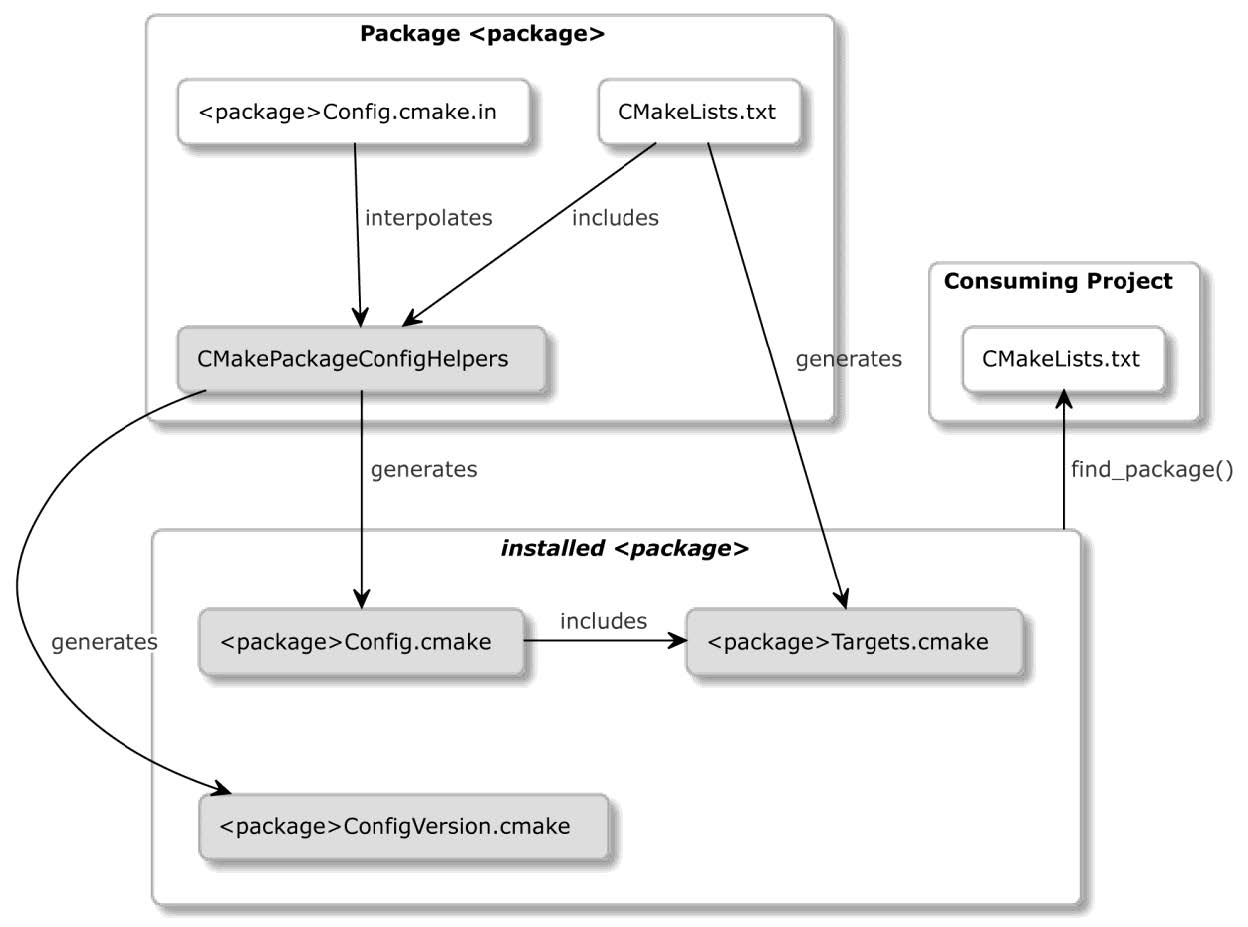
\includegraphics[width=0.8\textwidth]{content/3/chapter11/images/1.jpg}\\
Figure 11.1 – The file structure for advanced packages
\end{center}

All the required sub-dependencies of a package must also be found in the package config file. This can be done by calling the find\_dependency() macro from the CMakeFindDependencyMacro helper. We learned how to use it in Chapter 7, Managing Dependencies with CMake.

If you decide to expose any macros or functions to the consuming project, it is recommended that you put their definitions in a separate file that you can include() from the package's config-file.

Interestingly, CMakePackageConfigHelpers also provides a helper command to generate package's version files. Let's take a look.

\subsubsubsection{11.4.5\hspace{0.2cm}Generating package version files}

As your package grows, it will slowly gain new features, old ones will be marked as deprecated, and eventually be removed. It's important to keep track of these modifications in a changelog that's available to developers that use your package. When a specific feature is needed, a developer can find the lowest version that supports it and use it as an argument to find\_package(), like so:

\begin{lstlisting}[style=styleCMake]
find_package(Calc 1.2.3 REQUIRED)
\end{lstlisting}

CMake will then search the config-file for Calc and check if a version file named <config-file>-version.cmake or <config-file>Version.cmake is present in the same directory, that is, CalcConfigVersion.cmake. Next, this file will be read for its version information and the compatibility it provides with other versions. For example, you may not have version 1.2.3 installed as required, but you may have 1.3.5, which is marked as "compatible" with any older versions. CMake will gladly accept such a package as it knows that the package vendor provides backward compatibility.

You can use the CMakePackageConfigHelpers utility module to generate package's version files by calling write\_basic\_package\_version\_file():

\begin{lstlisting}[style=styleCMake]
write_basic_package_version_file(<filename> [VERSION <ver>]
	COMPATIBILITY <AnyNewerVersion | SameMajorVersion |
				   SameMinorVersion | ExactVersion>
	[ARCH_INDEPENDENT]
)
\end{lstlisting}

First, we need to provide the <filename> property of the artifact we want to create; it must follow the rules we outlined earlier. Other than that, keep in mind that we should store all the generated files in the build tree.

Optionally, we can pass an explicit VERSION (the usual format, major.minor.patch, is supported here). If we don't do this, the version that's provided in the project() command will be used instead (expect an error if your project doesn't specify one).

The COMPATIBILITY keyword is self-explanatory:

\begin{itemize}
\item 
ExactVersion must match all three components of the version and won't support ranged versions: find\_package(<package> 1.2.8...1.3.4).

\item 
SameMinorVersion matches if the first two components are the same (ignores patch).

\item 
SameMajorVersion matches if the first component is the same (ignores minor and patch).

\item 
AnyNewerVersion seems to have a reversed name: it will match any older version. In other words, <package> on version 1.4.2 will be a good match for find\_package(<package> 1.2.8).
\end{itemize}

Normally, all packages must be built for the same architecture as the consuming project to match (an exact check is performed). However, for packages that don't compile anything (header-only libraries, macro packages, and so on), you can specify the ARCH\_INDEPENDENT keyword to skip this check.

Now, it's time for a practical example. The following code shows how to provide the version file for the project that we started in the 06-install-export example:

\begin{lstlisting}[style=styleCMake]
# chapter-11/10-version-file/CMakeLists.txt (fragment)

cmake_minimum_required(VERSION 3.20.0)
project(VersionFile VERSION 1.2.3 LANGUAGES CXX)
...
include(CMakePackageConfigHelpers)
write_basic_package_version_file(
	"${CMAKE_CURRENT_BINARY_DIR}/CalcConfigVersion.cmake"
	COMPATIBILITY AnyNewerVersion
)
install(FILES "CalcConfig.cmake"
	"${CMAKE_CURRENT_BINARY_DIR}/CalcConfigVersion.cmake"
	DESTINATION ${CMAKE_INSTALL_LIBDIR}/calc/cmake
)
\end{lstlisting}

For convenience, we configure the version of the package at the top of the file, in the project() command. This requires us to switch from the short project(<name> <languages>) syntax to an explicit, full syntax by adding the LANGUAGE keyword.

After including the helper utility module, we call the generation command and write the file to a build tree with a name conforming to the pattern that's required by find\_package(). Here, we deliberately skip the VERSION keyword to have the version read from the PROJECT\_VERSION variable. We're also marking our package as fully backward compatible with COMPATIBILITY AnyNewerVersion. After that, we install the package version file to the same destination as CalcConfig.cmake. And that's it – our package is fully configured.

In the next section, we'll learn what components are and how to use them with packages.







